% !TEX program = xelatex
% AI-effects 프로젝트 --- 점유율 지표 A·B·C 상위 30, 하위 30 엑셀 파일 설명.
% 표 본문: results/table/34_sheets.tex, 34_top10_ksco3.tex, 34_ksco1.tex, 34_notes.tex
%          (code/04_17_analysis_kor_share_top30.do가 생성)
% 설명 대상: results/table/34_kor_share_top30.xlsx, 34_kor_share_bottom30.xlsx
% 관련: paper 19(한국 업무용 대화 비중), 21(SOC 2018--KSCO 8차 연계표), 26(소분류 상위 30의 SOC 구성), 27(점유율 지표 A~D)
% 컴파일: xelatex 두 번 (kotex 필요)
\documentclass[11pt]{article}

\usepackage{fontspec}
\usepackage{kotex}
\usepackage[a4paper,margin=2.0cm]{geometry}
\usepackage{longtable}
\usepackage{booktabs}
\usepackage{array}
\usepackage{amsmath}
\usepackage{xcolor}
\usepackage{hyperref}
\usepackage{enumitem}
\usepackage{graphicx}

\hypersetup{colorlinks=true,linkcolor=blue!50!black,urlcolor=blue!50!black}
\newcolumntype{L}[1]{>{\raggedright\arraybackslash}p{#1}}
\newcolumntype{R}[1]{>{\raggedleft\arraybackslash}p{#1}}
\setlength{\LTleft}{0pt}
\setlength{\LTright}{0pt}
\renewcommand{\arraystretch}{1.15}
\setlength{\tabcolsep}{3.5pt}

\title{점유율 지표 A$\cdot$B$\cdot$C 상위 30$\cdot$하위 30 직업 엑셀 파일 설명\\[2mm]
\large --- SOC 세부 직업과 KSCO 세분류$\cdot$소분류$\cdot$중분류$\cdot$대분류 ---}
\author{AI-effects 프로젝트}
\date{\today}

\begin{document}
\maketitle

\begin{abstract}
\noindent 이 노트는 \texttt{results/table/34\_kor\_share\_top30.xlsx}(상위 30)와 \texttt{34\_kor\_share\_bottom30.xlsx}(하위 30)를 설명한다. 두 파일은 \texttt{code/04\_17\_analysis\_kor\_share\_top30.do}가 한 번에 만들고, 시트 구성과 열이 같다. 각 시트는 한 분류 단계에서 지표 하나로 직업을 줄 세운 목록이다. 분류 단계는 SOC 세부 직업, KSCO 8차 세분류$\cdot$소분류$\cdot$중분류$\cdot$대분류다. 지표는 paper 27의 점유율 지표 A(업무용 대화 점유율), B(절감 시간 점유율), C(취업자 환산 절감 점유율)다. KSCO 시트에는 그 직업의 값에 가장 많이 기여한 한 단계 아래 직업(기여 1위)과 그 몫을 함께 적었다.
\begin{itemize}[leftmargin=*]
  \item \textbf{시트 11개}: SOC 2개(A, B), 세분류 2개(A, B), 소분류 3개(A, B, C), 중분류 3개(A, B, C), 대분류 1개(9개 전부). 세분류에는 C가 없다. C의 분모인 1인당 근로시간이 소분류에만 있기 때문이다.
  \item \textbf{값은 다른 paper와 같다.} 소분류$\cdot$중분류$\cdot$대분류 값은 \texttt{03\_05}의 지표 그대로다. 세분류 값은 같은 규칙으로 새로 만들었고, 소분류 안 세분류를 더하면 소분류 값과 같다(do 파일에서 assert).
  \item \textbf{쏠림이 크다.} 상위 30개의 점유율 합은 SOC$\cdot$세분류에서 59$\sim$60\%, 소분류에서 81$\sim$84\%다. 소분류 1$\cdot$2위는 A에서 291 작가 및 언론 관련 전문가, 222 컴퓨터 시스템 및 소프트웨어 전문가이고, B$\cdot$C에서는 순서가 바뀐다.
  \item \textbf{하위 30은 해석에 주의가 필요하다.} 2026-11-01부터 한국 대화 비중이 공개되지 않은 직업도 사용 0으로 넣으므로, 소분류$\cdot$세분류의 하위 목록은 사용 0인 직업(소분류 34개, 세분류 151개)이 같은 값으로 채운다. 사용이 있는 직업 중 하위권은 값이 0.001\% 안팎으로 작아 AEI 공개 비중의 최소 단위, 한 달만 공개된 직업, 연계표에서 SOC 하나만 이어진 직업의 영향을 크게 받는다. 4절에 점검 수치를 모았다.
\end{itemize}
\end{abstract}

\section{두 파일과 시트 구성}

두 파일의 시트 이름과 열은 같다. 상위 파일은 값이 큰 순(첫 열 ``순위'', 1 = 가장 큼), 하위 파일은 값이 작은 순(첫 열 ``하위 순위'', 1 = 가장 작음)이다. 같은 값에는 평균 순위를 주고, 30번째와 같은 값을 가진 직업은 모두 목록에 넣는다(2026-11-01). 그래서 목록이 30개보다 길 수 있다(표 1의 목록 수). 대분류 시트(\texttt{ksco1})는 9개 전부를 담으므로 두 파일의 내용이 같고 정렬 방향만 다르다.

\begin{small}
\begin{longtable}{L{1.6cm}L{2.6cm}L{1.2cm}R{1.3cm}R{1.3cm}R{2.3cm}R{2.3cm}}
\caption{시트 구성: 대상 수와 목록에 든 직업의 점유율 합}\label{tab:sheets}\\
\toprule
시트 & 분류 단계 & 기준 지표 & 대상 수 & 목록 수(상위 / 하위) & 상위 목록 합(\%) & 하위 목록 합(\%) \\
\midrule
\endfirsthead
\toprule
시트 & 분류 단계 & 기준 지표 & 대상 수 & 목록 수(상위 / 하위) & 상위 목록 합(\%) & 하위 목록 합(\%) \\
\midrule
\endhead
% 04_17_analysis_kor_share_top30.do가 생성. 직접 고치지 말 것.
\texttt{soc\_A} & SOC 세부 직업 & 지표 A & 368 & 30 / 31 & 58.6 & 0.12 \\
\texttt{soc\_B} & SOC 세부 직업 & 지표 B & 368 & 30 / 30 & 59.8 & 0.04 \\
\texttt{ksco4\_A} & KSCO 세분류 & 지표 A & 489 & 30 / 151 & 59.6 & 0.00 \\
\texttt{ksco4\_B} & KSCO 세분류 & 지표 B & 489 & 30 / 151 & 60.2 & 0.00 \\
\texttt{ksco3\_A} & KSCO 소분류 & 지표 A & 163 & 30 / 34 & 81.3 & 0.00 \\
\texttt{ksco3\_B} & KSCO 소분류 & 지표 B & 163 & 30 / 34 & 84.1 & 0.00 \\
\texttt{ksco3\_C} & KSCO 소분류 & 지표 C & 163 & 30 / 34 & 84.4 & 0.00 \\
\texttt{ksco2\_A} & KSCO 중분류 & 지표 A & 56 & 30 / 30 & 98.0 & 3.17 \\
\texttt{ksco2\_B} & KSCO 중분류 & 지표 B & 56 & 30 / 30 & 98.9 & 1.73 \\
\texttt{ksco2\_C} & KSCO 중분류 & 지표 C & 56 & 30 / 30 & 98.9 & 1.88 \\
\texttt{ksco1} & KSCO 대분류 & 지표 A & 9 & 9 / 9 & 100.0 & 100.00 \\

\bottomrule
\end{longtable}
\end{small}

각 시트의 열은 다음과 같다(요청 목록 순서).
\begin{itemize}[leftmargin=*]
  \item \texttt{soc\_A}, \texttt{soc\_B}: 순위, SOC 코드, SOC 직업명(BLS), 기준 지표, 다른 지표(A 시트는 A, B 순, B 시트는 B, A 순).
  \item \texttt{ksco4\_A}, \texttt{ksco4\_B}: 순위, KSCO 세분류 코드, 직업명, 기준 지표, 다른 지표, 기여 1위 SOC, 그 몫(\%).
  \item \texttt{ksco3\_*}, \texttt{ksco2\_*}: 순위, 코드, 직업명, 기준 지표, 나머지 두 지표, 기여 1위 하위 직업(소분류 시트는 세분류, 중분류 시트는 소분류), 그 몫(\%).
  \item \texttt{ksco1}: 지표 A 순위, 코드, 직업명, A, B, C, B 순위, C 순위, 지표별 기여 1위 중분류와 그 몫(\%) 세 쌍.
\end{itemize}
엑셀의 값은 반올림하지 않은 \% 값이다. 직업명은 SOC는 BLS 영문 명칭, KSCO는 통계청 명칭이다.

\section{지표 정의}

기간은 AEI 한국 자료의 2026년 4월과 5월이다. 두 달은 월별 비중을 구한 뒤 단순평균했고, 공개되지 않은 달은 0으로 두었다(paper 19, 27과 같은 규칙).

\paragraph{SOC 세부 직업.} 지표 A는 한국 업무용 대화 중 그 SOC의 비중이다.
\[
\text{A}_s = 100 \times \tfrac{1}{2} \sum_t \text{share\_work}_{st}
\]
지표 B는 업무용 비중에 대화당 절감 시간(AEI GLOBAL 값, 분)을 곱한 값 $\text{saved\_w}_{st}$의 점유율이다.
\[
\text{B}_s = 100 \times \tfrac{1}{2} \sum_t \frac{\text{saved\_w}_{st}}{\sum_{s'} \text{saved\_w}_{s't}}
\]
A는 농림어업 세부 직업 미공개 몫을 모은 자리표시 행 45-XXXX까지 더해 100이다. 45-XXXX는 순위에서 뺐다. 이 행에는 절감 시간이 없어 B에는 처음부터 들어가지 않는다.

\paragraph{KSCO 세분류(4자리).} SOC 단계 값을 SOC 2018--KSCO 8차 연계표의 배분 몫 $w_{sk}$(paper 21의 \texttt{w\_alloc})로 나눠 붙였다.
\[
\text{A}_k = 100 \times \tfrac{1}{2} \sum_t \frac{\sum_s \text{share\_work}_{st}\, w_{sk}}{T^{A}_t}, \qquad
\text{B}_k = 100 \times \tfrac{1}{2} \sum_t \frac{\sum_s \text{saved\_w}_{st}\, w_{sk}}{T^{B}_t}
\]
$T_t$는 \texttt{03\_05}가 소분류 163개(사용 0인 34개 포함)로 정규화할 때 쓴 월 $t$의 합이다. 그래서 소분류 안 세분류 값을 더하면 소분류의 A, B와 정확히 같다. 대상은 163개 소분류에 속한 세분류 489개 전부다. 이 중 338개는 연결된 SOC 중 한국 비중이 공개된 것이 있고, 151개는 없어 사용 0이다(기여 1위 빈칸).

\paragraph{KSCO 소분류$\cdot$중분류$\cdot$대분류.} \texttt{kor\_ai\_usage\_ksco\{3,2,1\}}의 \texttt{shA}, \texttt{shB}, \texttt{shC}를 그대로 썼다(paper 27). 지표 C는 B를 소분류의 1인당 월 주업 근로시간(지역별고용조사 2022 상반기)으로 나눠 다시 정규화한 값이다. 즉 절감 시간을 일하는 사람 수로 바꾼 점유율이다. 중분류$\cdot$대분류 값은 소분류 값의 합이다.

\paragraph{기여 1위.} 시트의 기준 지표로 정한다.
\begin{itemize}[leftmargin=*]
  \item 세분류 $\leftarrow$ SOC: A 시트는 $\text{share\_work} \times w_{sk}$, B 시트는 $\text{saved\_w} \times w_{sk}$가 가장 큰 SOC.
  \item 소분류 $\leftarrow$ 세분류: A 시트는 세분류 A, B$\cdot$C 시트는 세분류 B가 가장 큰 세분류. 소분류 안에서는 1인당 근로시간이 같으므로 C의 몫은 B의 몫과 같다.
  \item 중분류 $\leftarrow$ 소분류, 대분류 $\leftarrow$ 중분류: 각 지표 값이 가장 큰 하위 직업.
\end{itemize}
몫(\%)은 기여 1위의 값을 그 직업 값으로 나눈 것이다. 50\%를 넘으면 그 직업의 값은 사실상 하위 직업 하나가 정한다.

\section{결과 개관}

\begin{small}
\begin{longtable}{R{0.5cm}L{4.0cm}R{1.0cm}L{4.0cm}R{1.0cm}L{4.0cm}R{1.0cm}}
\caption{KSCO 소분류 상위 10: 지표 A, B, C(\%)}\label{tab:top10}\\
\toprule
 & 지표 A 순 & A & 지표 B 순 & B & 지표 C 순 & C \\
\midrule
\endfirsthead
% 04_17_analysis_kor_share_top30.do가 생성. 직접 고치지 말 것.
1 & 291 작가 및 언론 관련 전문가 & 11.92 & 222 컴퓨터 시스템 및 소프트웨어 전문가 & 12.21 & 222 컴퓨터 시스템 및 소프트웨어 전문가 & 11.56 \\
2 & 222 컴퓨터 시스템 및 소프트웨어 전문가 & 9.95 & 291 작가 및 언론 관련 전문가 & 10.47 & 291 작가 및 언론 관련 전문가 & 11.08 \\
3 & 225 정보 시스템 및 웹 운영자 & 8.32 & 225 정보 시스템 및 웹 운영자 & 5.34 & 372 비서 및 사무 지원 종사자 & 5.81 \\
4 & 372 비서 및 사무 지원 종사자 & 4.69 & 372 비서 및 사무 지원 종사자 & 5.24 & 225 정보 시스템 및 웹 운영자 & 5.13 \\
5 & 283 상품 기획‧홍보 및 조사 전문가 & 4.20 & 283 상품 기획‧홍보 및 조사 전문가 & 5.15 & 283 상품 기획‧홍보 및 조사 전문가 & 5.06 \\
6 & 223 네트워크 및 정보 보안 전문가 & 3.84 & 332 통계‧데이터 관련 사무원 & 4.03 & 332 통계‧데이터 관련 사무원 & 4.20 \\
7 & 292 학예사‧사서 및 기록물 관리사 & 3.81 & 223 네트워크 및 정보 보안 전문가 & 3.74 & 213 생명 및 자연과학 관련 시험원 & 3.51 \\
8 & 213 생명 및 자연과학 관련 시험원 & 2.79 & 213 생명 및 자연과학 관련 시험원 & 3.62 & 223 네트워크 및 정보 보안 전문가 & 3.51 \\
9 & 332 통계‧데이터 관련 사무원 & 2.61 & 211 생명 및 자연과학 관련 전문가 & 2.89 & 293 연극‧영화 및 영상 전문가 & 2.91 \\
10 & 340 금융 사무 종사자 & 2.61 & 293 연극‧영화 및 영상 전문가 & 2.85 & 211 생명 및 자연과학 관련 전문가 & 2.78 \\

\bottomrule
\end{longtable}
\end{small}

소분류 상위 10은 정보 통신$\cdot$글쓰기$\cdot$사무 지원$\cdot$연구 직업으로 세 지표가 거의 같다. 차이는 대화당 절감 시간에서 나온다(paper 31). 225 정보 시스템 및 웹 운영자는 A 3위(8.32\%)지만 대화당 절감 시간이 짧아 B 5.34\%로 줄어든다. 332 통계$\cdot$데이터 관련 사무원은 반대로 A 9위에서 B$\cdot$C 6위로 오른다. C는 B를 1인당 근로시간으로 나눈 값이라 B와 순서가 거의 같다. 372 비서 및 사무 지원 종사자는 225보다 1인당 근로시간이 짧아 C에서 225를 앞서 3위가 된다. 상위 30 겹침은 A와 B, A와 C 모두 26개다(표~\ref{tab:notes}).

그림~\ref{fig:top30}은 \texttt{ksco3\_C} 시트의 상위 30 전체를 막대로 그린 것이다. 1$\cdot$2위(222, 291)가 각각 11\% 남짓으로 3위 이하의 두 배가 넘고, 막대 색으로 보면 상위 30 대부분이 전문가(대분류 2)이며 사무(3)와 관리자(1)가 그 뒤를 잇는다.
\begin{figure}[htbp]
\centering
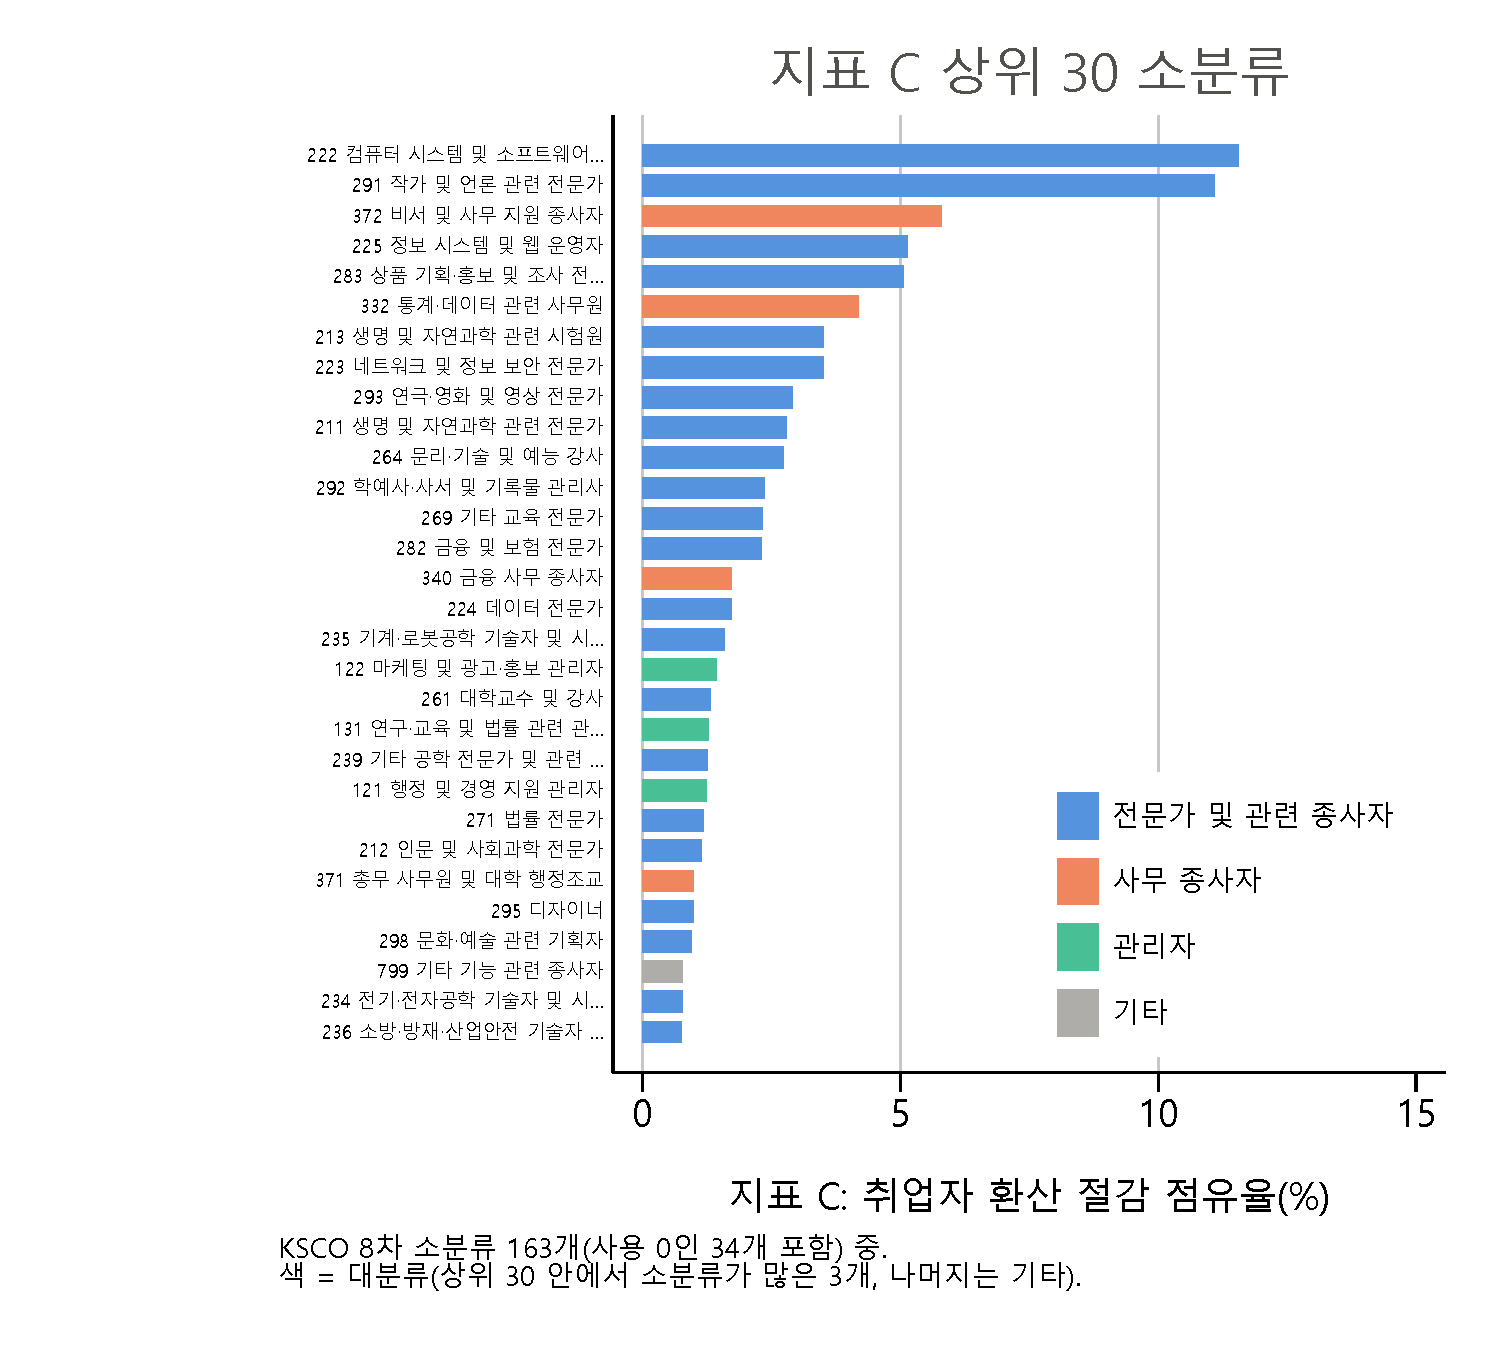
\includegraphics[width=0.85\textwidth]{../figure/34_fig_ksco3_top30_C.pdf}
\caption{지표 C 상위 30 소분류(색 = 대분류)}\label{fig:top30}
\end{figure}


\begin{small}
\begin{longtable}{R{0.4cm}L{4.4cm}R{1.2cm}R{1.6cm}R{1.6cm}L{6.0cm}}
\caption{KSCO 대분류: 지표 A, B, C(\%, 괄호는 순위)와 지표 A 기여 1위 중분류(몫, \%)}\label{tab:ksco1}\\
\toprule
 & 대분류 & A & B & C & 지표 A 기여 1위 중분류 \\
\midrule
\endfirsthead
% 04_17_analysis_kor_share_top30.do가 생성. 직접 고치지 말 것.
1 & 2 전문가 및 관련 종사자 & 70.50 & 72.18 (1) & 71.88 (1) & 22 정보 통신 전문가 및 기술직 (33.8) \\
2 & 3 사무 종사자 & 14.64 & 14.40 (2) & 15.05 (2) & 37 일반 지원 사무직 (41.1) \\
3 & 1 관리자 & 6.86 & 8.89 (3) & 8.37 (3) & 13 전문 서비스 관리직 (39.7) \\
4 & 5 판매 종사자 & 3.17 & 1.25 (5) & 1.20 (5) & 52 매장 판매 및 상품 대여직 (60.2) \\
5 & 7 기능원 및 관련 기능 종사자 & 1.94 & 1.42 (4) & 1.55 (4) & 79 기타 기능 관련직 (43.6) \\
6 & 4 서비스 종사자 & 1.10 & 0.52 (7) & 0.60 (7) & 41 경찰‧소방 및 보안 관련 서비스직 (34.5) \\
7 & 8 장치∙기계 조작 및 조립 종사자 & 0.88 & 0.97 (6) & 0.88 (6) & 85 기계 제조‧관련 기계 조작 및 조립직 (72.7) \\
8 & 9 단순노무 종사자 & 0.88 & 0.36 (8) & 0.47 (8) & 99 농림어업 및 기타 서비스 단순 노무직 (53.0) \\
9 & 6 농림∙어업 숙련 종사자 & 0.03 & 0.00 (9) & 0.00 (9) & 61 농축산 숙련직 (78.7) \\

\bottomrule
\end{longtable}
\end{small}

대분류에서는 전문가 및 관련 종사자가 A$\cdot$B$\cdot$C의 70\% 이상을 차지하고, 그 안에서 22 정보 통신 전문가 및 기술직의 몫이 가장 크다. 관리자는 B$\cdot$C에서 A보다 몫이 커지고, 판매$\cdot$서비스$\cdot$단순노무는 줄어든다. 9개 중 6개는 세 지표의 기여 1위 중분류가 같다. 다른 지표의 기여 1위는 \texttt{ksco1} 시트에 있다.

\section{읽을 때 유의사항}

\begin{longtable}{L{12.5cm}R{2.5cm}}
\caption{하위 목록과 기여 1위를 읽을 때 쓰는 점검 수치}\label{tab:notes}\\
\toprule
항목 & 값 \\
\midrule
\endfirsthead
% 04_17_analysis_kor_share_top30.do가 생성. 직접 고치지 말 것.
SOC 지표 A 최솟값(\%) / 그 값을 가진 SOC 수 & 0.00124 / 6 \\
SOC 지표 B 최솟값(\%) / 그 값을 가진 SOC 수 & 0.00017 / 1 \\
세분류 지표 A 상위 30 중 기여 1위 SOC 몫이 50\% 이상인 수 & 23 \\
세분류 지표 A 하위 30 중 기여 1위 SOC 몫이 100\%(SOC 하나)인 수 & 30 \\
세분류 전체 중 기여 1위 SOC 몫이 100\%인 수 & 115 / 338 \\
소분류 중 한 달만 공개된 수 & 7 \\
소분류 하위 30 중 한 달만 공개된 수(A / B / C) & 7 / 7 / 7 \\
소분류 상위 30 겹침(A와 B / A와 C) & 26 / 26 \\
대분류 중 A·B·C 기여 1위 중분류가 모두 같은 수 & 6 / 9 \\

\bottomrule
\end{longtable}

\begin{enumerate}[leftmargin=*]
  \item \textbf{SOC 지표 A의 하위권에는 동점이 있다.} 최솟값 0.00124\%를 가진 SOC가 6개다. 이 값은 AEI가 공개한 한국 비중의 최소 단위로 보인다(공개 규칙은 확인하지 않았다). 동점에는 평균 순위를 주므로 지표 A 하위 목록은 31개다. B는 SOC별 절감 시간을 곱하므로 최솟값을 가진 SOC가 하나뿐이다.
  \item \textbf{소분류 하위 목록은 사용 0인 34개다}(A, B, C 모두, 평균 순위 146.5위로 동점). 한 달만 공개된 소분류 7개는 그 바로 위, 사용이 있는 소분류의 하위권에 있다. 비공개 달을 0으로 두고 두 달을 평균했기 때문에 값이 공개된 달의 절반이다. 이 소분류의 하위 순위는 사용이 적다는 뜻과 한 달만 공개됐다는 뜻이 섞여 있다.
  \item \textbf{세분류 기여 1위는 연계표 배분을 그대로 보여 준다.} 세분류 489개 중 115개는 한국 비중이 공개된 SOC가 하나뿐이어서 기여 1위 몫이 100\%다. 사용 0인 151개는 기여 1위가 없다. 이전 판(338개)에서는 하위 30이 모두 몫 100\%였지만, 지금 하위 목록은 사용 0인 151개다. 예를 들어 9412 운송 및 시설장비 청소원과 9991 구두 미화원의 기여 1위는 39-4012 Crematory Operators이고, 2133 자연과학 시험원의 지표 B 기여 1위는 15-2051 Data Scientists다. 이런 연결은 연계표의 단계별 배분(paper 21)과, AEI 직업이 사용자의 직업이 아니라 대화 과업의 직업이라는 점에서 생긴다. 직업 간 비교에 쓰기 전에 연계 경로를 확인해야 한다.
  \item \textbf{SOC 시트와 KSCO 시트의 합은 기준이 다르다.} SOC 값은 한국 업무용 대화 전체(45-XXXX 포함) 중 비중이고, KSCO 값은 소분류 163개(사용 0인 34개는 0) 안에서 다시 정규화한 비중이다. 같은 대화라도 SOC 시트와 KSCO 세분류 시트의 숫자를 직접 더하거나 빼지 않는다.
  \item \textbf{절감 시간은 추정치다.} B$\cdot$C의 대화당 절감 시간은 AEI가 대화마다 추정한 ``사람이 혼자 하면 걸릴 시간'' $-$ ``AI와 함께 걸린 시간''의 GLOBAL 평균이다. 한국 대화에도 같은 값을 썼다.
  \item \textbf{점유율은 수준이 아니다.} 모든 값은 한국 업무용 AI 대화(또는 절감 시간) 안에서의 몫이다. 직업 규모 대비 사용 강도는 상대 활용도 RU1$\cdot$RU2(paper 25, 32)로 본다.
\end{enumerate}

\section{산출 파일}

\begin{itemize}[leftmargin=*]
  \item 코드: \texttt{code/04\_17\_analysis\_kor\_share\_top30.do}(Stata 17, \texttt{00\_master.do}에 포함). 입력은 \texttt{kor\_soc6\_conv\_ai\_indicators}(\texttt{03\_03}), SOC 2018--KSCO 8차 연계표(\texttt{01\_06}), \texttt{kor\_ai\_usage\_ksco\{3,2,1\}}(\texttt{03\_05}).
  \item 엑셀: \texttt{results/table/34\_kor\_share\_top30.xlsx}, \texttt{34\_kor\_share\_bottom30.xlsx}(시트 11개씩).
  \item 이 노트의 표: \texttt{results/table/34\_sheets.tex}, \texttt{34\_top10\_ksco3.tex}, \texttt{34\_ksco1.tex}, \texttt{34\_notes.tex}.
  \item 그림: \texttt{results/figure/34\_fig\_ksco3\_top30\_C.\{pdf,png\}}(\texttt{code/04\_20\_analysis\_kor\_share\_figures.do}).
\end{itemize}

\end{document}
